%実験・結果
本章では,本研究における実験内容及び結果について述べる.

%1節
\section{実験内容}
遅延故障シミュレータにFF制御を実装し,検出率を算出する.
本実験では,全体の10\%のFFを制御した.
FF制御を行う場合と行わない場合それぞれにおいて,
遅延故障検出率の観点から性能差を比較する.
今回実験に用いた回路の詳細は表5.1の通りである.
\begin{table}[htb]
 \begin{center}
 \caption{実験回路情報}
  \begin{tabular}{|l|r|r|r|} \hline
    回路名 & s5378 & s9234 & s13207 \\ \hline \hline
    信号線の数 & 5344本 & 9256本 & 13300本 \\
    FFの総数 & 179個 & 228個 & 669個 \\
    制御するFFの数 & 17個 & 22個 & 66個 \\ \hline
  \end{tabular}
  \end{center}
\end{table}

3種類すべての回路において,テストパターン数100でシミュレーションを行い,
2サイクルから10サイクルにかけての遅延故障検出率の推移を算出した.
なお,本研究で使用されたプログラムはすべてC言語で開発されている.

%2節
\section{実験結果}
それぞれの回路における遅延故障検出率を以下の図に示す.
図では,FF制御なしのグラフは青線で,FF制御ありのグラフは黄線で表している.
得られた結果に対する考察は次章にて述べる.

\begin{figure}[h]
\begin{center}
	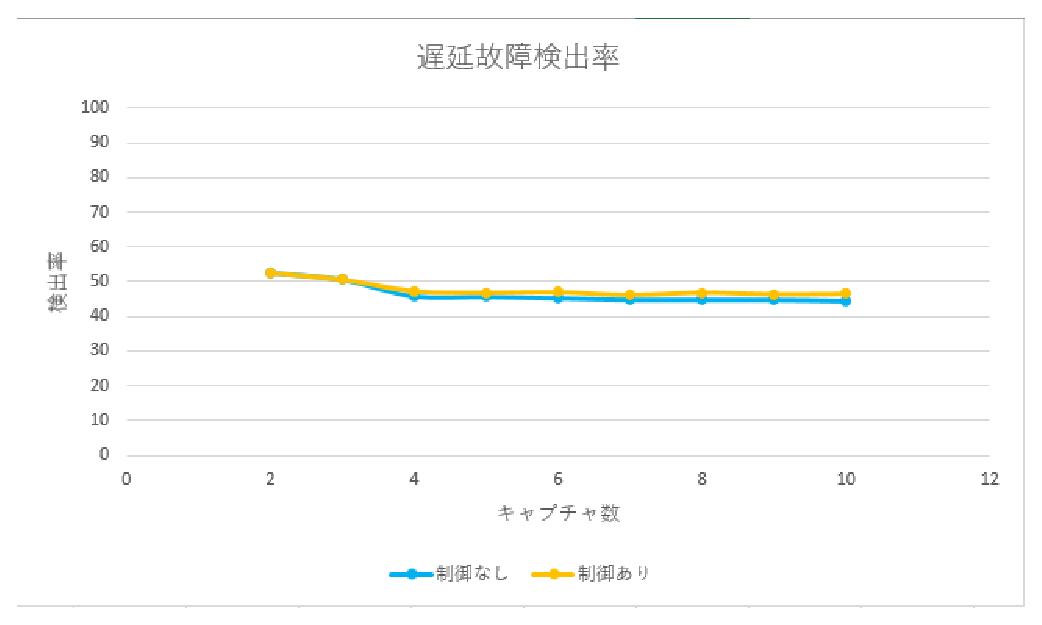
\includegraphics[height=80mm]{s5378CPI.eps}
	\caption{s5378回路における遅延故障検出率}
\end{center}
\end{figure}

\begin{figure}[h]
\begin{center}
	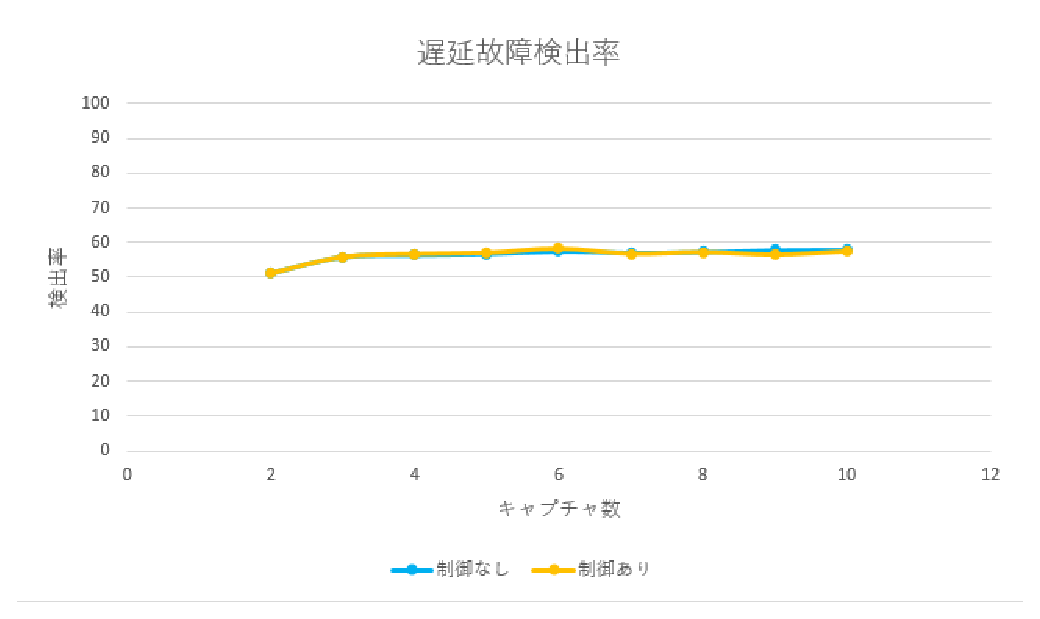
\includegraphics[height=80mm]{s9234CPI.eps}
	\caption{s9234回路における遅延故障検出率}
\end{center}
\end{figure}

\begin{figure}[h]
\begin{center}
	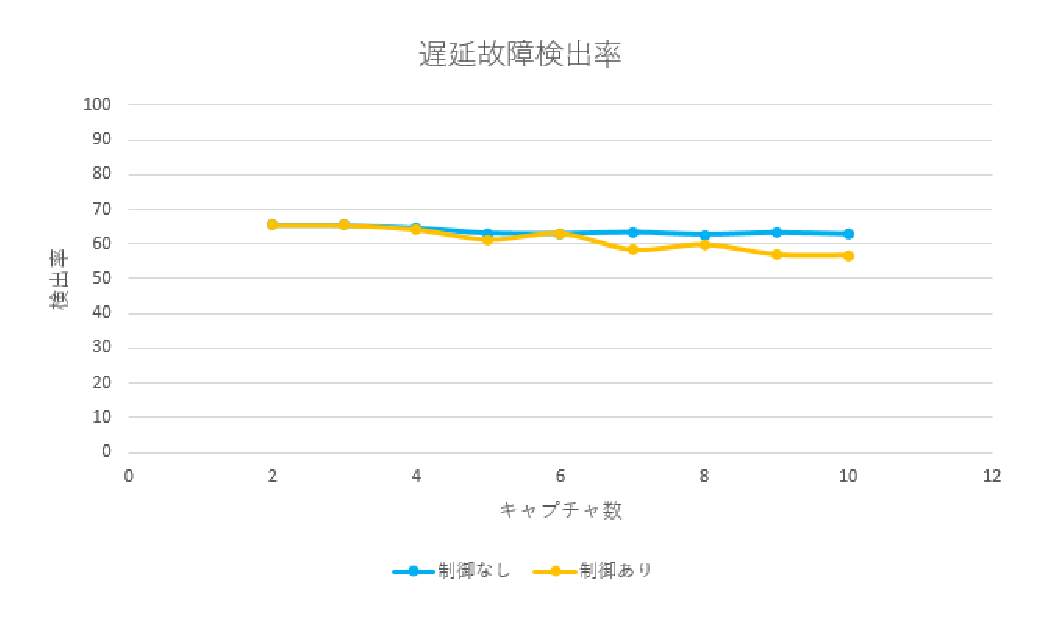
\includegraphics[height=80mm]{s13207CPI.eps}
	\caption{s13207回路における遅延故障検出率}
\end{center}
\end{figure}